\addcontentsline{toc}{section}{\numberline {1}Inhaltsverzeichnis}
\addcontentsline{toc}{section}{\numberline {2}Originalangabe}
\setcounter{section}{2} \setcounter{page}{2}

\includepdf[angle=-90]{res/doc/Angabe.jpg}

\section{Plichtenheft}
	Es soll für den Mikrocontroller für ein LCD-Display (EADOGM204A) eine Library in C geschrieben werden, damit
	dieses anschließend über SPI angesteuert und verwendent werden kann. Deswegen soll ein Datenblatt vom Hersteller gesucht werden 
	und mit den dort gefundenen Informationen soll dann mnit der Software begonnen werden. Die Funktionsfähigkeit der Library soll 
	am Tag der Abgabe anhand eines kleinen Testprogramms nachgewiesen werden. Die Library soll ohne detailliertes Vorwissen
	über die Hardware, verwendet werden können.

\section{Zeitablaufdiagramm}
	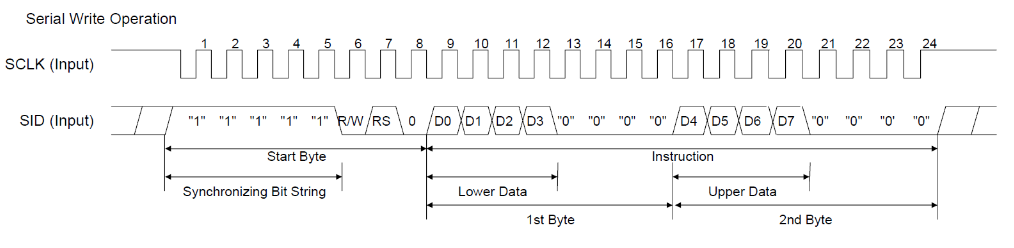
\includegraphics[width=\textwidth]{res/img/Zeitablaufdiagramm.PNG}
	
\section{Kommentiertes Listing}
	\UseRawInputEncoding
	\subsection{LCD.h}
		{\scriptsize\lstinputlisting[language={c}]{res/src/LCD.h}}
	\subsection{LCD.c}
		{\scriptsize\lstinputlisting[language={c}]{res/src/LCD.c}}
	\subsection{main.c}
		{\scriptsize\lstinputlisting[language={c}]{res/src/main.c}}
	\inputencoding{utf8}
	
\section{Zeitaufwand}
	\subsubsection*{Robert Radu:}
		\begin{tabular}{|$l|^l|}
			\hline
			\rowstyle{\bfseries} Tätigkeit                                    & Aufwand \\\hline
			                     Erstellung des Plichtenhefts                 & 1h      \\\hline
			                     Programmcodierung                            & 5h      \\\hline
			                     Testen der Software                          & 0.5h      \\\hline
			                     Dokumentation (Protokoll)                    & 0.5h      \\\hline
			\rowstyle{\bfseries} Gesamt                                       & 7h      \\\hline
		\end{tabular}
		
	\subsubsection*{Paul Raffer:}
		\begin{tabular}{|$l|^l|}
			\hline
			\rowstyle{\bfseries} Tätigkeit                                    & Aufwand \\\hline
			                     Erstellung des Plichtenhefts                 & 0h      \\\hline
			                     Programmcodierung                            & 7h     \\\hline
			                     Testen der Software                          & 1h    \\\hline
			                     Dokumentation (Protokoll)                    & 2h      \\\hline
			\rowstyle{\bfseries} Gesamt                                       & 10h      \\\hline
		\end{tabular}
		
\section{Aufgetretene Probleme}
	\begin{tabular}{|$l|^l|}
		\hline
		\rowstyle{\bfseries} Problem & Lösung                                           \\\hline
		                     \textbackslash n soll eine neue Zeile ausgeben & nicht gelöst \\\hline
	\end{tabular}
		
\addcontentsline{toc}{section}{Anhang}
	\addcontentsline{toc}{subsection}{Messprotokoll}
	\addcontentsline{toc}{subsection}{Datenblatter (Command Table)}
	
\includepdf[pages=-,angle=-90]{res/doc/Messprotokoll.jpg}
\includepdf[pages={38,39,40}]{res/doc/Datenblaetter/ssd1803a_2_0.pdf}
